\chapter{Performence}

web性能速度是关键,而影响速度主要就是延时和带宽两方面的影响。

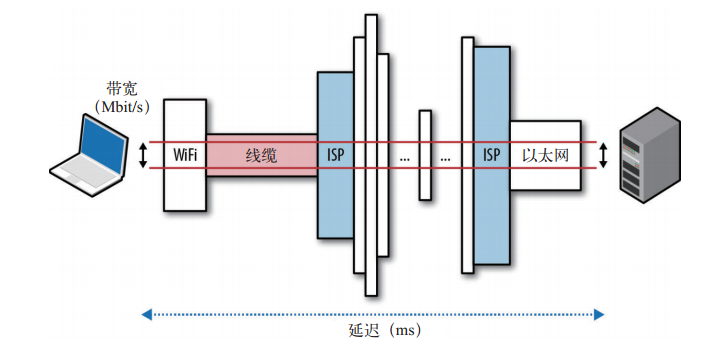
\includegraphics[scale=1]{web/resources/delay-band.png}


\begin{itemize}
\item 延时,分组从信息源发送到目的地的时间;
\begin{itemize}
\item 传播延时,消息从发送端到接收端的时间,与信号传播距离和速度有关。

CDN(Content Delivery Network),最主要用途就是将内容部署到全球各地,让用户从最近的服务器加载内容。

延时的最后一公里。


\item 传输延时,消息的所有bit转移到链路中所需要的时间,与消息长度和链路速率有关。
\item 处理延时,处理分组首部,检查位错误,确定分组目标所需要的时间。
\item 排队延时,到来分组排队等待的时间。
\end{itemize}
\item 带宽,逻辑或者物理通信线路的最大吞吐量。
\end{itemize}



\section{TCP}

\subsubsection{三次握手}

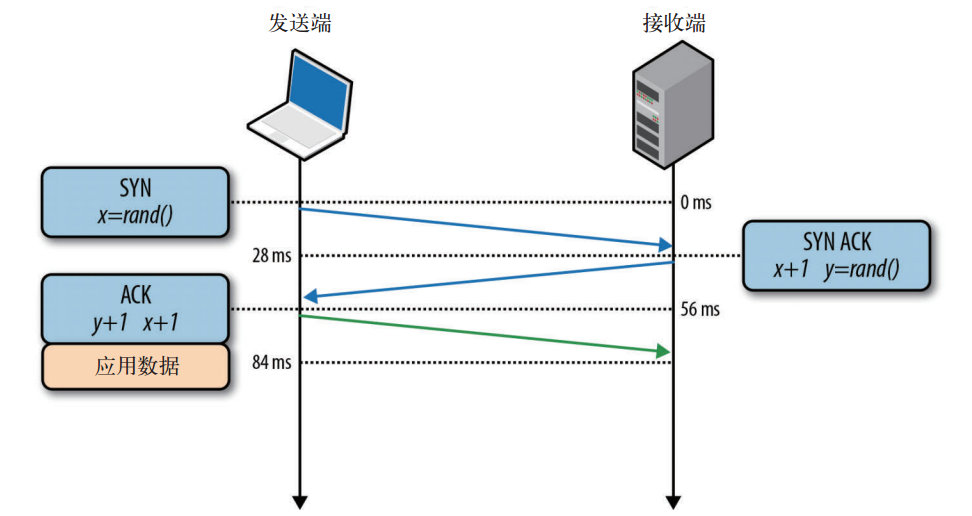
\includegraphics[scale=1]{web/resources/TCP-3-hand-shake.png}

\begin{itemize}
\item SYN,客服端选择随机数(ISN)一个SYN发送给客服端,
\item SYN/ACK,服务器响应ACK(SYN+1),同时选择自己的随机数发送给客服端
\item ACK,客服端发送ACK(服务器端的SYN+1)
\end{itemize}

三次握手的延时使得创建一个新的TCP连接的代价非常大。所以提高TCP应用的性能的关键是,重用连接。

\subsubsection{拥塞预防与控制}

\paragraph{rwnd}TCP连接的双方都会通告自己的接收窗口(rwnd)

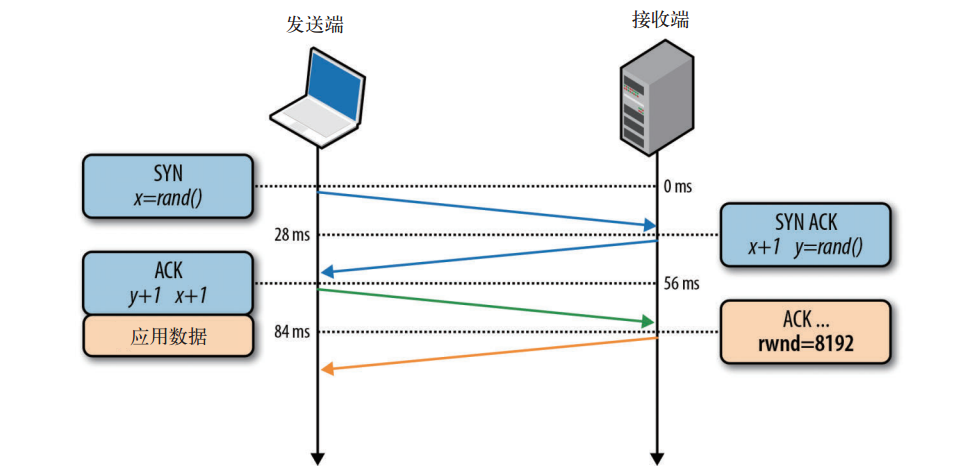
\includegraphics[scale=1]{web/resources/TCP-rwnd.png}

第一次建立连接是,双方都会使用系统默认设置来发送rwnd。浏览网页主要是从服务器向客服端发送数据,这样客服端的窗口可能会成为瓶颈。而上传图片或者视频,是客服端向服务器发送大量数据,服务器的接收窗口又可能成为制约因素。

窗口缩放。

\paragraph{慢启动}

拥塞窗口变量(cwnd),

\paragraph{队首阻塞}


\subsubsection{总结}

\begin{itemize}
\item 三次握手增加了整整一次往返时间。(因为的三次ACK可以携带应用数据)
\item 慢启动应用到每个连接
\item 流量及拥塞控制会影响到连接的吞吐量
\item 吞吐量由当前拥塞窗口的大小控制。
\end{itemize}

\section{UDP}

\section{Wireless}

\section{HTTP}

\section{Web API}